\subsection{Merge Sort}

\begin{figure}[h]
	\centering
	\mbox{
		\subfigure[Test results from Merge Sort when run in .NET.]{
			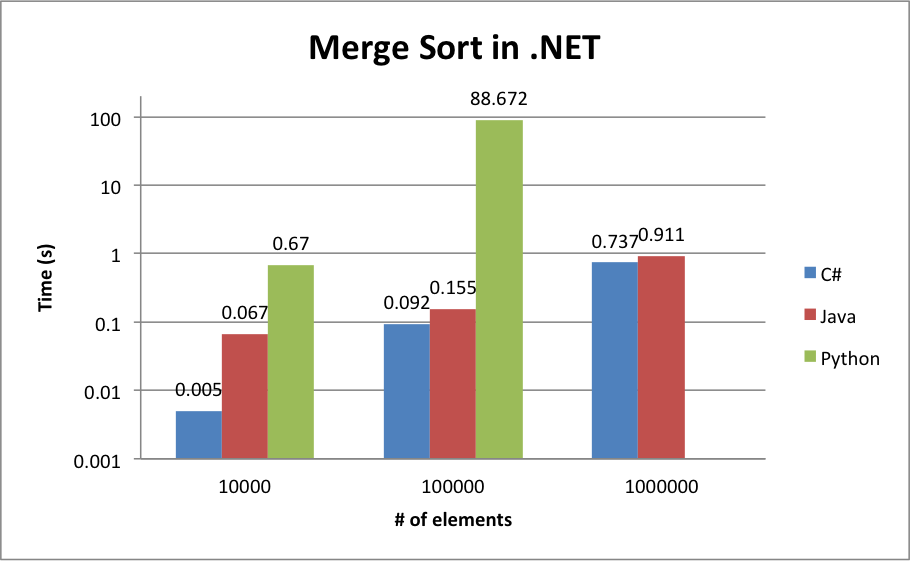
\includegraphics[width=0.48\textwidth]{chapters/media/merge_sort_all_net.png}
			\label{fig:merge_sort_all_net}
		}
		\subfigure[Test results from Merge Sort when run in native environments.]{
			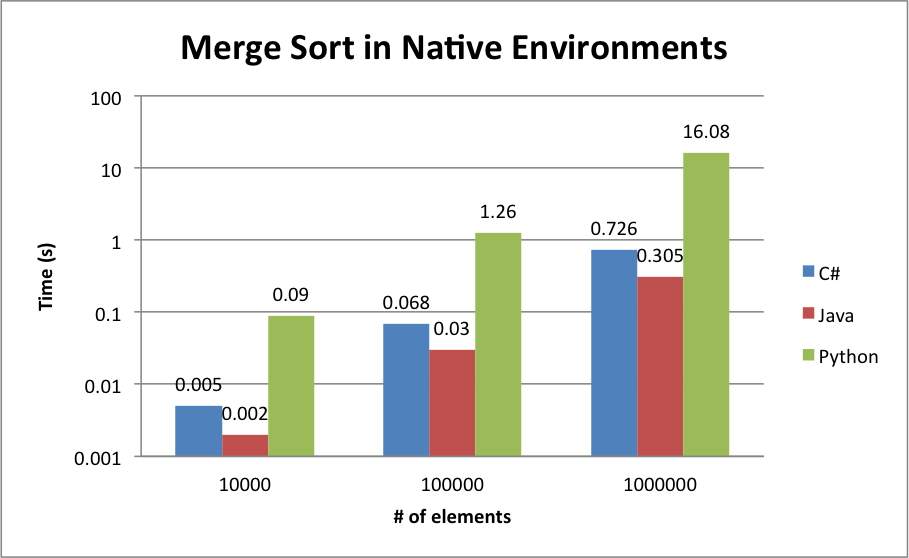
\includegraphics[width=0.48\textwidth]{chapters/media/merge_sort_all_native.png}
			\label{fig:merge_sort_all_native}
		}
	}
	\caption{Comparison of running Merge Sort in .NET to the left and each language native environment to the right.}
	\label{fig:merge_sort_net_native}
\end{figure}


Since the runtime for Python was already over the one minute mark with just 100'000 elements (see Figure \ref{fig:merge_sort_all_net}) I decided not to test one million elements with Python. Instead I tested C\# and Java with one million elements and compared the runtimes with one hundred thousand elements in Figure \ref{fig:merge_sort_csharp_java}.

\begin{figure}[h]
	\centering
	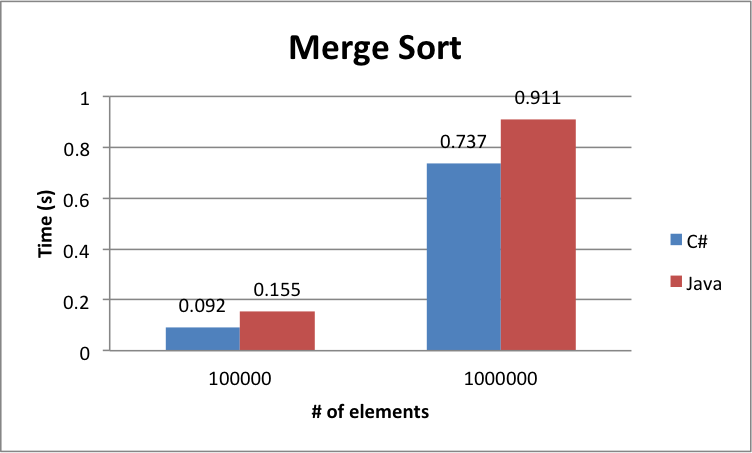
\includegraphics[width=0.6\textwidth]{chapters/media/merge_sort_csharp_java.png}
	\caption{Time difference between using 100'000 elements and a million.}
	\label{fig:merge_sort_csharp_java}
\end{figure}

C\# still outperforms Java when run in the .NET environment. But the gap between them seemed to narrow the more elements were added. I attempted to run the Java implementation in its native environment, and it  outperformed C\# (see Figure \ref{fig:merge_sort_csharp_java_native}). 

\begin{figure}[h]
	\centering
	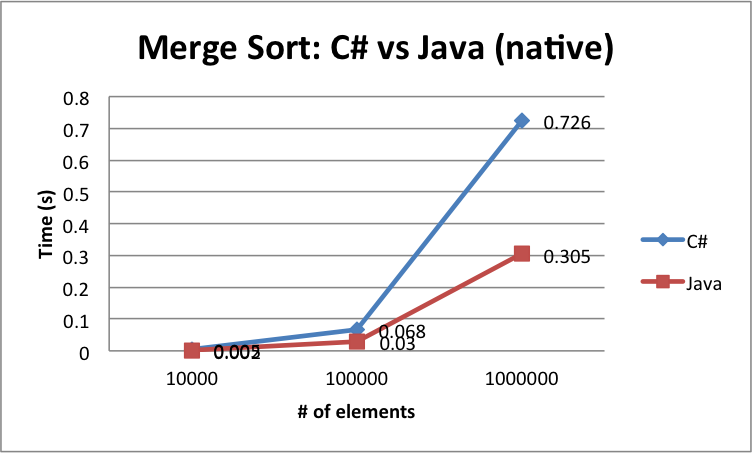
\includegraphics[width=0.6\textwidth]{chapters/media/merge_sort_csharp_java_native.png}
	\caption{Comparing Java and C\# when both are run in their respective native environments.}
	\label{fig:merge_sort_csharp_java_native}
\end{figure}

\begin{figure}[h]
	\centering
	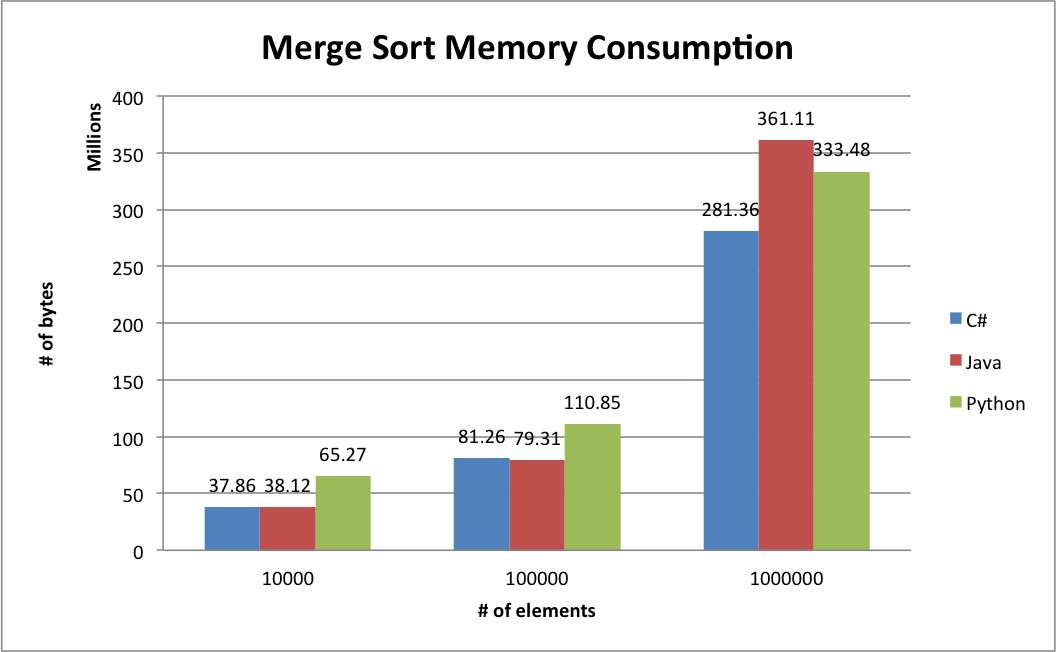
\includegraphics[width=0.6\textwidth]{chapters/media/merge_sort_memory.png}
	\caption{Comparing Java and C\# when both are run in their respective native environments.}
	\label{fig:merge_sort_memory}
\end{figure}

Java run in .NET is about equal to C\# when it comes to memory management (Figure \ref{fig:merge_sort_memory}). Python consumed more memory, performing 40-50\% worse than the other two.


\begin{figure}[h]
	\centering
	\mbox{
		\subfigure[Java under the .NET Environment and the native environment.]{
			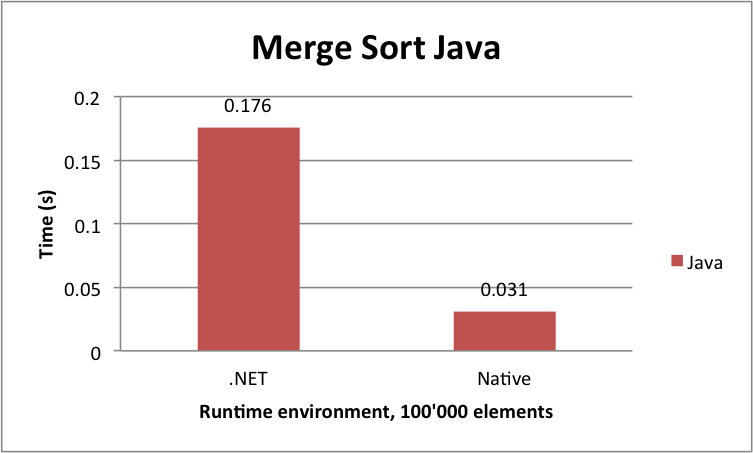
\includegraphics[width=0.48\textwidth]{chapters/media/merge_sort_java_native.png}
			\label{fig:merge_sort_native_java}
		}
		\subfigure[Python under the .NET Environment and the native environment.]{
			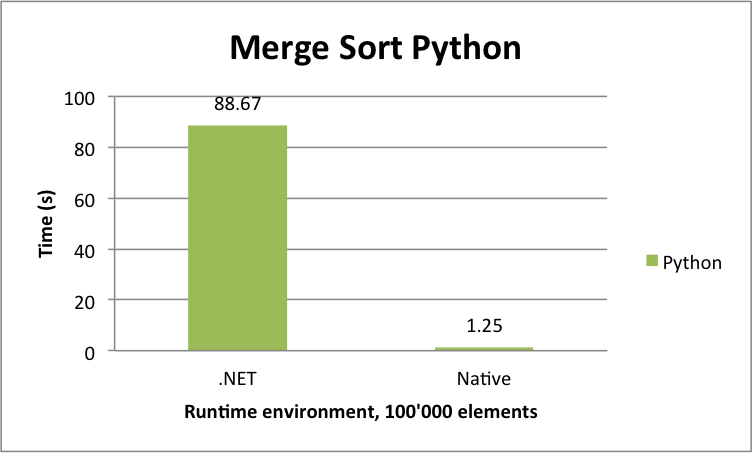
\includegraphics[width=0.48\textwidth]{chapters/media/merge_sort_python_native.png}
			\label{fig:merge_sort_native_python}
		}
	}
	\caption{Comparison of running under the .NET Environment and the native environment with Java to the left and Python to the right (using 100'000 elements).}
	\label{fig:merge_sort_natives}
\end{figure}

Running code in its native environment provides a big increase in performance for Merge Sort as well. Java is about 5-6 times faster and Python is more than 70 times faster (see Figure \ref{fig:merge_sort_natives}). The slow execution of Python code in .NET seem to depend on the size of the input as seen in Figure blsblalbla FIXME. 























